\documentclass[11pt, a4paper]{article}
\usepackage{graphicx}
\usepackage{amsmath}
\usepackage{listings}
\usepackage{color}
\usepackage{fancyhdr}
\usepackage[utf8]{inputenc}
\usepackage[%  
    colorlinks=true,
    pdfborder={0 0 0},
    linkcolor=red
]{hyperref}

\definecolor{dkgreen}{rgb}{0,0.6,0}
\definecolor{gray}{rgb}{0.5,0.5,0.5}
\definecolor{mauve}{rgb}{0.58,0,0.82}

\lstset{frame=tb,
  language=Python,
  aboveskip=3mm,
  belowskip=3mm,
  showstringspaces=false,
  columns=flexible,
  basicstyle={\small\ttfamily},
  numbers=none,
  numberstyle=\tiny\color{gray},
  keywordstyle=\color{blue},
  commentstyle=\color{dkgreen},
  stringstyle=\color{mauve},
  breaklines=true,
  breakatwhitespace=true,
  tabsize=3
}

\title{Assignment 5}
\author{Manvar Nisharg EE19B094}
\date{March 22 2021}
\setlength{\headheight}{15pt}
\pagestyle{fancy}
\fancyhf{}
\rhead{Assignment - 5}
\lhead{EE2703 - Applied Programming Lab}
\rfoot{Page \thepage}

\usepackage{natbib}
\usepackage{graphicx}
\usepackage{amsmath}
\usepackage{listings}

\begin{document}

\maketitle
\newpage

\begin{abstract}
    In this assignment we want to visualise the currents in a resistor. We will also see which part of the resistor becomes the hottest due to the currents.
\end{abstract}


\section{Setup}
A  cylindrical wire is soldered to the middle of a copper plate of dimension 1cm by 1cm. Voltage of the wire is held at 1 Volt.  Bottom side of the plate is grounded, while the remaining are kept floating.\newline\newline
Consider the following results:\newline
\begin{equation}
    \nabla \cdot \vec{j} = - \frac{\partial\rho}{\partial t}
\end{equation}
\begin{equation}
    \vec{j} = \sigma\vec{E}
\end{equation}
\begin{equation}
    \vec{E} = -\nabla\phi
\end{equation}
From the above equations:
\begin{equation}
    \nabla^2 \phi =  \frac{1}{\rho}\frac{\partial\rho}{\partial t}
\end{equation}
Now, For DC Currents, RHS of equation (3) is 0. Hence:
\begin{equation}\label{eqn(5)}
    \nabla^2 \phi =  0
\end{equation}


\section{Defining Parameters}
We have chosen a 25x25 grid with a circle of radius 8 centrally located which represents the wire whose $V = 1V$ always. We ask the user for the arguments and in case they are not appropriate we choose the default values.

\begin{lstlisting}
#User Input else default
try:
    if(len(sys.argv)==5):
        Nx=int(sys.argv[1])
        Ny=int(sys.argv[2])
        radius=int(sys.argv[3])  
        Niter=int(sys.argv[4])
    else:
        print("Invalid format of parameters given in commandline")
        Nx=25 # length along x
        Ny=25 # length along y
        radius=8 #radius of central lead
        Niter=1500 #number of iterations
except:
    print("Invalid format of parameters given in commandline")
    Nx=25 # length along x
    Ny=25 # length along y
    radius=8 #radius of central lead
    Niter=1500 #number of iterations
\end{lstlisting}

\section{Finding Potential Matrix}
\subsection{ Initializing Potential Matrix}
We represent the grid of data points of size Nx x Ny using a matrix of same size. We initialize it with 0 and then we find the points lying withing the circle of radius 8 and initialize them to 1. We then plot its contour plot.
\begin{lstlisting}
#initialize potential matrix
phi_matrix=np.zeros((Nx,Ny),dtype = float)
#Range of points on X and Y axis
x_range,y_range=np.linspace(-0.5,0.5,num=Nx,dtype=float), np.linspace(-0.5,0.5,num=Ny,dtype=float)
Y,X=np.meshgrid(y_range,x_range,sparse=False)   #Make grid from x and y values
phi_matrix[np.where(X**2+Y**2<(0.35)**2)]=1.0   #Make electorde voltage as 1V

#Contour plot for initial potential
plt.title("Initial potential contour plot")
plt.contourf(X,Y,phi_matrix,cmap=plt.get_cmap('coolwarm'))
plt.xlabel(r"X$\longrightarrow$")
plt.ylabel(r"Y$\longrightarrow$")
plt.colorbar()
plt.show()
\end{lstlisting}
\begin{figure}[h!]
\centering
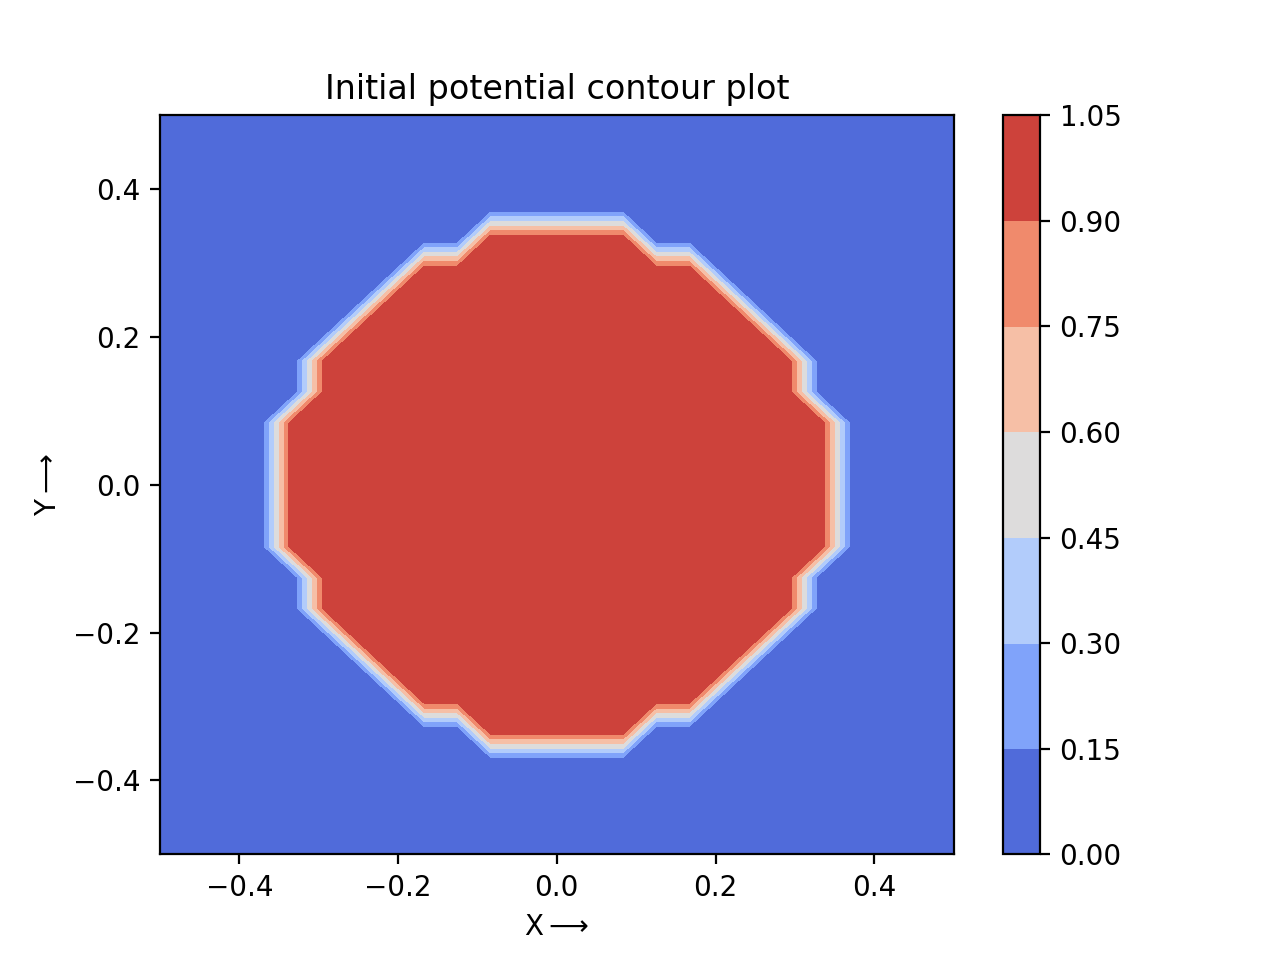
\includegraphics[scale=0.6]{Fig-1.png}
\caption{Initial Potential}
\label{fig:initial Potential}
\end{figure}
\newpage

\subsection{Iterating and Updating potential}
\subsubsection{Updating matrix}
We use the constraint given by Equation \ref{eqn(5)} to update the values of potential. However the equation is in differential form which we convert to discrete form 
.But Equation (4) is a differential equation. We need to first convert it to a difference equation as all of our code is in discrete domain.
We write it as :
\begin{equation}
    \phi_{i,j} = 0.25*(\phi_{i-1,j} + \phi_{i+1,j} + \phi_{i,j+1} + \phi_{i,j-1})
\end{equation}
\begin{lstlisting}
#Function to update voltage matrix for every iteration
def update_phi_voltage(phi_matrix,phiold):
    phi_matrix[1:-1,1:-1]=0.25*(phiold[1:-1,0:-2]+ phiold[1:-1,2:]+ phiold[0:-2,1:-1] + phiold[2:,1:-1])
    return phi_matrix
\end{lstlisting}

\subsubsection{Applying Boundary Conditions}
As no currents flows out of the top,left,right boundary the gradient at the potential at boundary must be 0. Also the bottom boundary is grounded. We apply this boundary condition after every iteration
\begin{lstlisting}
#Function to set the boundary conditions on voltage matrix for every iteration
def set_boundary_conditions_voltage(phi_matrix):
    phi_matrix[:,Nx-1]=phi_matrix[:,Nx-2] # Right Boundary
    phi_matrix[:,0]=phi_matrix[:,1] # Left Boundary
    phi_matrix[0,:]=phi_matrix[1,:] # Top Boundary
    phi_matrix[Ny-1,:]=0    #Grounded
    center = np.where(X**2+Y**2<(0.35)**2)
    phi_matrix[center]=1.0  #Make electorde voltage as 1V
    return phi_matrix
\end{lstlisting}

\subsubsection{Calculating error and running iterations}
We find the error between two iterations by taking the maximum of the absolute differences between corresponding data entries of the old and updated voltage matrices.
\begin{lstlisting}
#Initialize error matrix
error = np.zeros(Niter)
#Iterate and update the voltage matrix
for iteration in range(Niter):
    phiold = phi_matrix.copy()
    phi_matrix = update_phi_voltage(phi_matrix,phiold)  #Update matrix
    phi_matrix = set_boundary_conditions_voltage(phi_matrix)    #Set boundary condition
    error[iteration] = np.max(np.abs(phi_matrix-phiold))    #Error between old and new voltage matrix
    if(error[iteration] == 0):  #Break if error reaches steady state
        break
\end{lstlisting}


\clearpage
\subsection{Plotting and Fitting the error}
We see that the errors decreases pretty slowly with iterations and thus we plot them on semilogy and loglog plots.

We also observe that the error decreases in exponential form and thus we fit the error on a exponential and also plot that alongside the original error plot. However the exponential decay is only after around 500 iterations. Thus we plot two fits, one considering the error values of all the iterations and other with only after 500 iterations.
\begin{lstlisting}

#Function to get exponential fit for the error plot
def get_exponential_fit(y,Niter,iteration_start):
    log_error = np.log(error)[-iteration_start:]
    X = np.vstack([(np.arange(Niter)+1)[-iteration_start:], np.ones(log_error.shape)]).T
    log_error = np.reshape(log_error,(1,log_error.shape[0])).T
    return s.lstsq(X, log_error)[0]

#Function to plot the error
def plot_error(error,Niter,A1,A2,B1,B2):
    plt.title("Best fit for error on loglog scale")
    plt.xlabel(r"Iterations$\longrightarrow$")
    plt.ylabel(r"Error$\longrightarrow$")
    x = np.asarray(range(Niter))+1
    plt.loglog(x,error,label="Error")
    plt.loglog(x[::100],np.exp(A1+B1*np.asarray(range(Niter)))[::100],'ro',label="fit1")
    plt.loglog(x[::100],np.exp(A2+B2*np.asarray(range(Niter)))[::100],'go',label="fit2")
    plt.legend()
    plt.show()
    
    plt.title("Best fit for error on semilog scale")
    plt.xlabel(r"Iterations$\longrightarrow$")
    plt.ylabel(r"Error$\longrightarrow$")
    plt.semilogy(x,error,label="Error")
    plt.semilogy(x[::100],np.exp(A1+B1*np.asarray(range(Niter)))[::100],'ro',label="fit1")
    plt.semilogy(x[::100],np.exp(A2+B2*np.asarray(range(Niter)))[::100],'go',label="fit2")
    plt.legend()
    plt.show()

#Expoential fit with all entries
B1,A1 = get_exponential_fit(error,Niter,0)
#Expoential fit with entries only after 500 iterations
B2,A2 = get_exponential_fit(error,Niter,500)
plot_error(error,Niter,A1,A2,B1,B2)
\end{lstlisting}
\begin{figure}[h!]
\centering
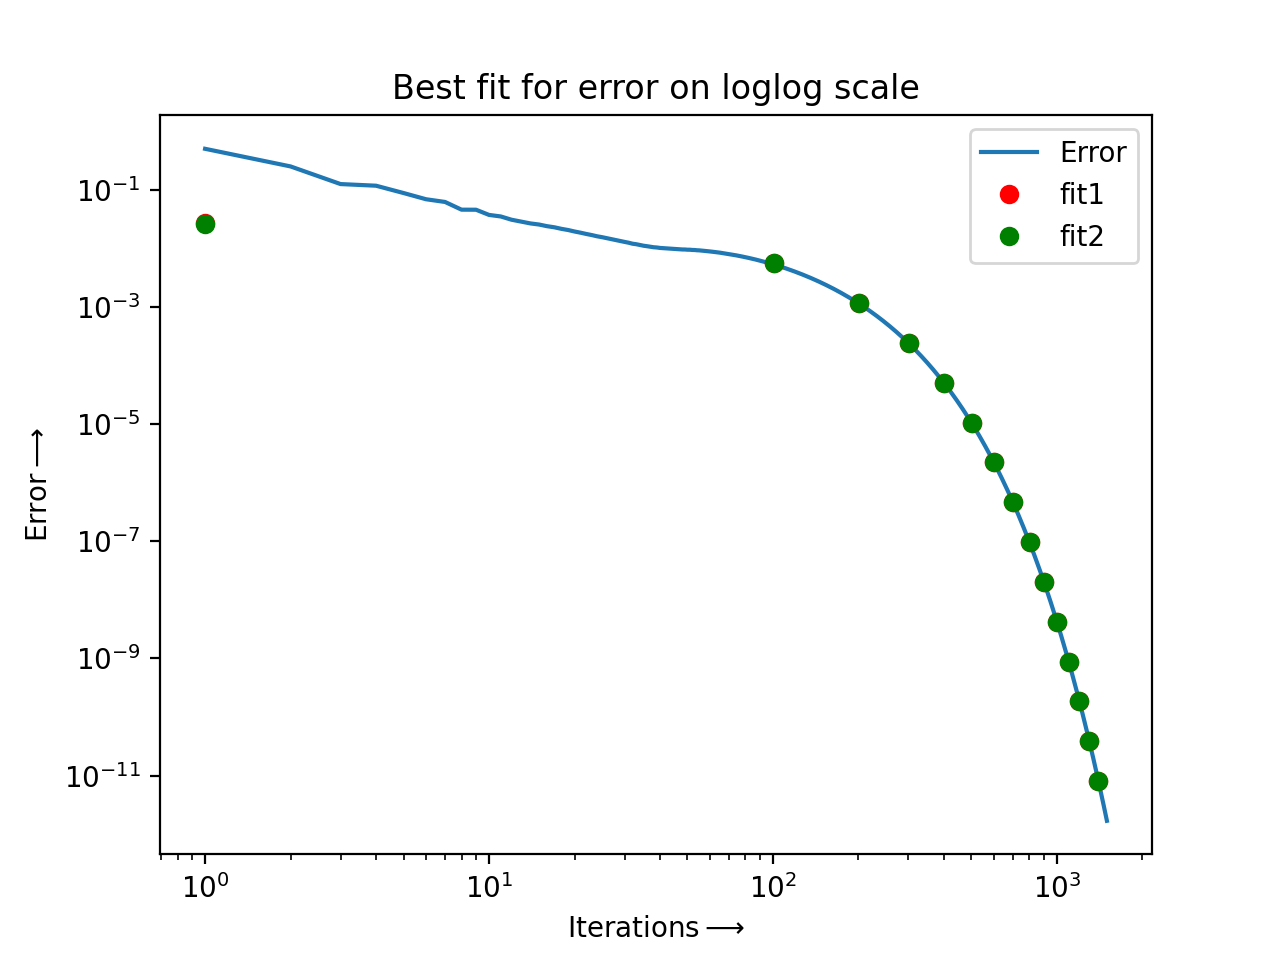
\includegraphics[scale=0.6]{Fig-2.png}
\caption{Best Fit of error}
\label{fig:Best Fit of error}
\end{figure}
\begin{figure}[h!]
\centering
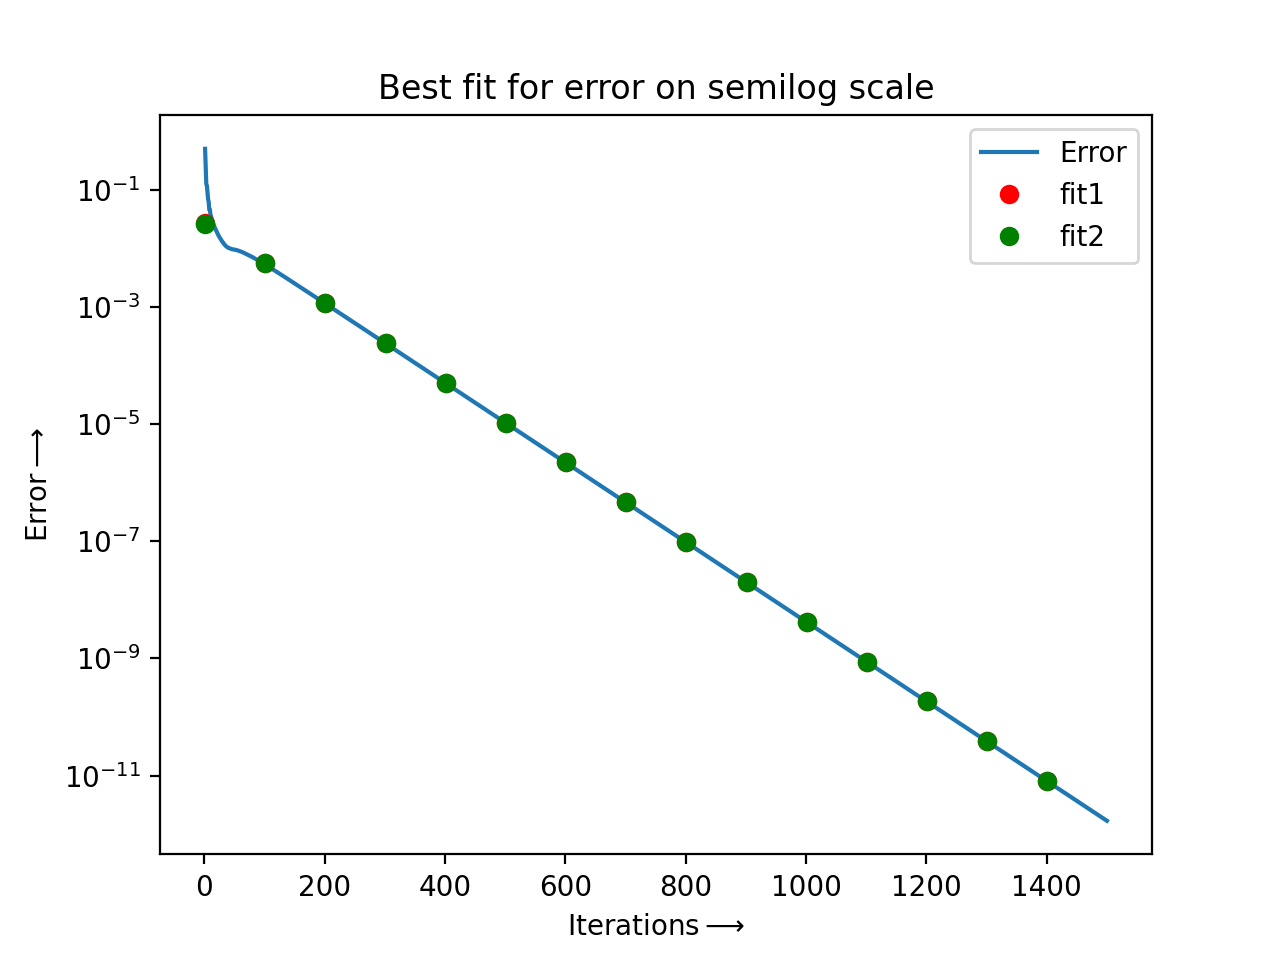
\includegraphics[scale=0.6]{Fig-3.png}
\caption{Best Fit of error}
\label{fig:Best Fit of error}
\end{figure}

\subsection{Plotting Max Cumulative Error}
As we saw in the previous section, the error reduces pretty slowly and thus this way of solving the Laplace's Equation is one of the worst possible methods. We can see in the following graph of max error on loglog scale that how slow it reduces.
\begin{lstlisting}
#Function to find net error
find_net_error = lambda a,b,Niter : -a/b*np.exp(b*(Niter+0.5))


#plotting cumulative error
iteration=np.arange(100,1501,100)
plt.grid(True)
plt.title(r'Cumulative Error on loglog scale')
plt.xlabel(r"Iterations$\longrightarrow$")
plt.ylabel(r"Net maximum error$\longrightarrow$")
plt.loglog(iteration,np.abs(find_net_error(A2,B2,iteration)),'ro')
plt.show()
\end{lstlisting}
\begin{figure}[h!]
\centering
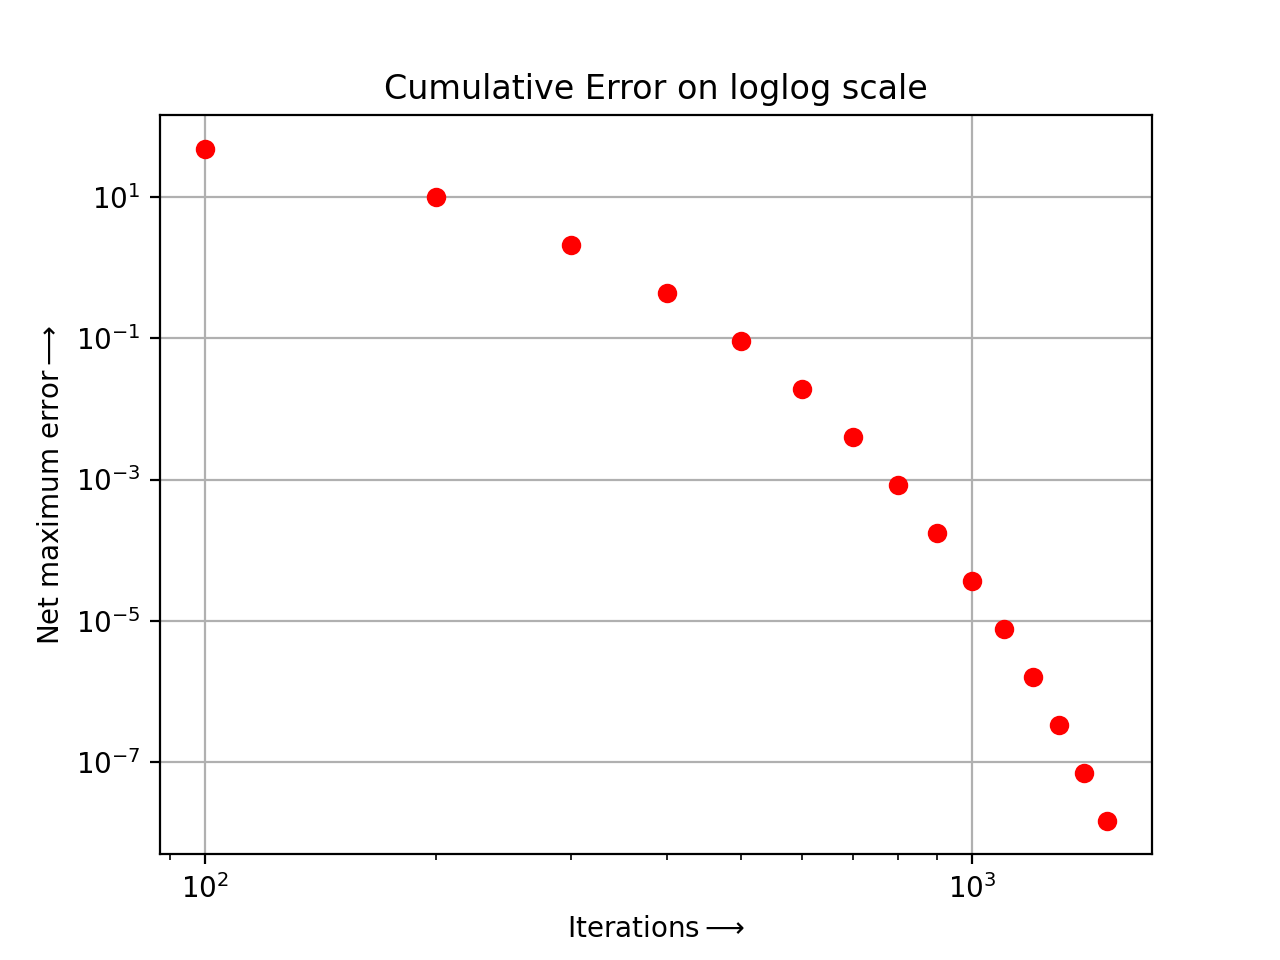
\includegraphics[scale=0.6]{Fig-4.png}
\caption{Cumulative error values on a log log scale}
\label{fig:3d Plot of Potential}
\end{figure}

\subsection{Plotting final voltage matrix}
\begin{lstlisting}
#plotting 2d contour of final potential
plt.title("2D Contour plot of final potential")
plt.xlabel(r"X$\longrightarrow$")
plt.ylabel(r"Y$\longrightarrow$")
plt.contourf(Y,X[::-1],phi_matrix)  #Contour plot
x_electrode,y_electrode=np.where(X**2+Y**2<(0.35)**2)   #Points with electode
plt.plot((x_electrode-Nx/2)/Nx,(y_electrode-Ny/2)/Ny,'ro')  #Mark those points as red
plt.colorbar()
plt.show()


#Plotting 3d contour of final potential
fig1=plt.figure(4)     # open a new figure
ax=p3.Axes3D(fig1) # Axes3D is the means to do a surface plot
plt.title('The 3-D surface plot of the final potential')
surf = ax.plot_surface(Y, X, phi_matrix.T, rstride=1, cstride=1, cmap=plt.cm.jet)
plt.show()
\end{lstlisting}

\begin{figure}[h!]
\centering
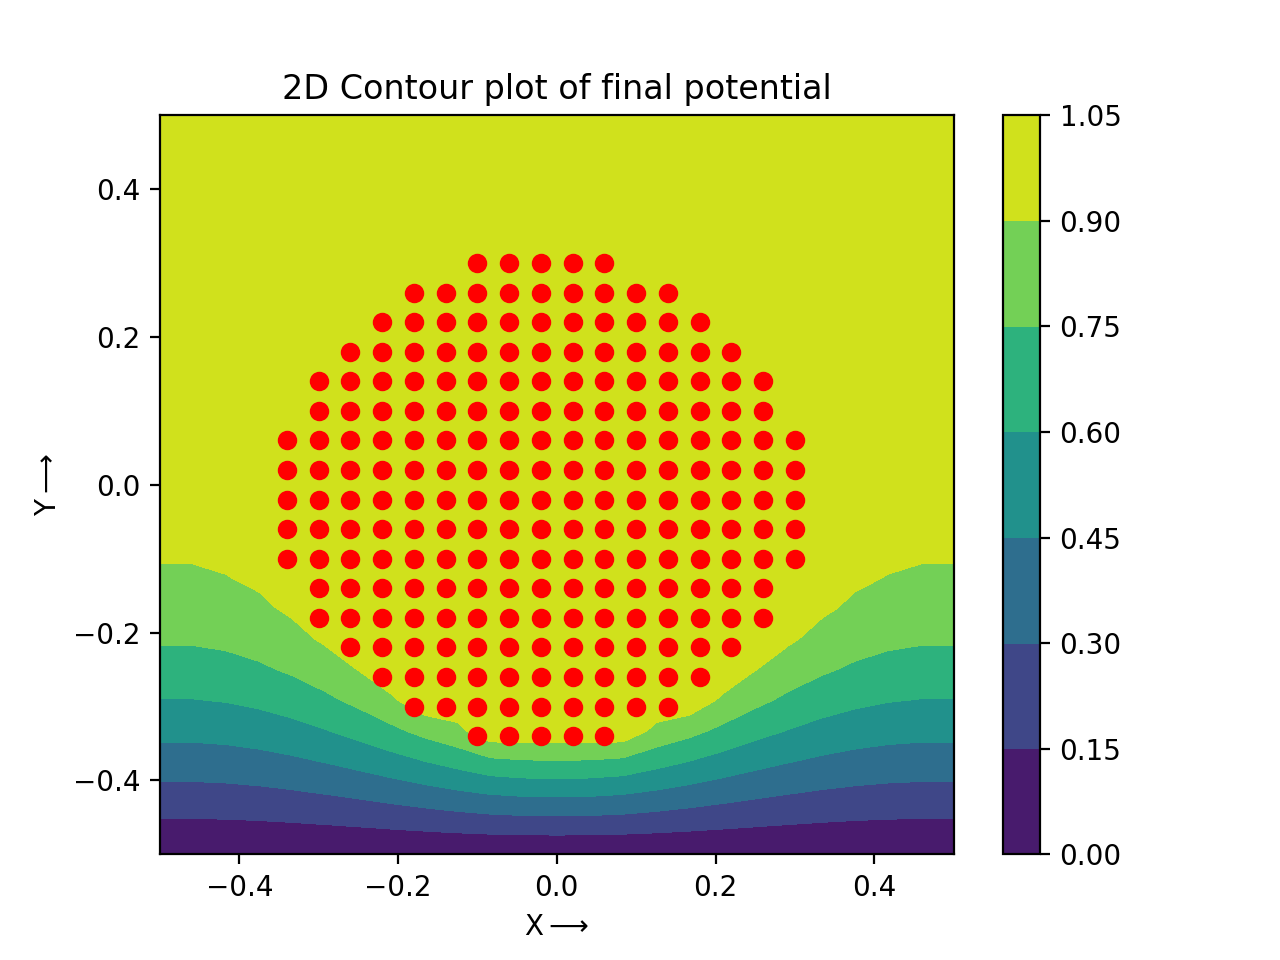
\includegraphics[scale=0.6]{Fig-5.png}
\caption{2d Plot of Potential}
\label{fig:3d Plot of Potential}
\end{figure}


\begin{figure}[h!]
\centering
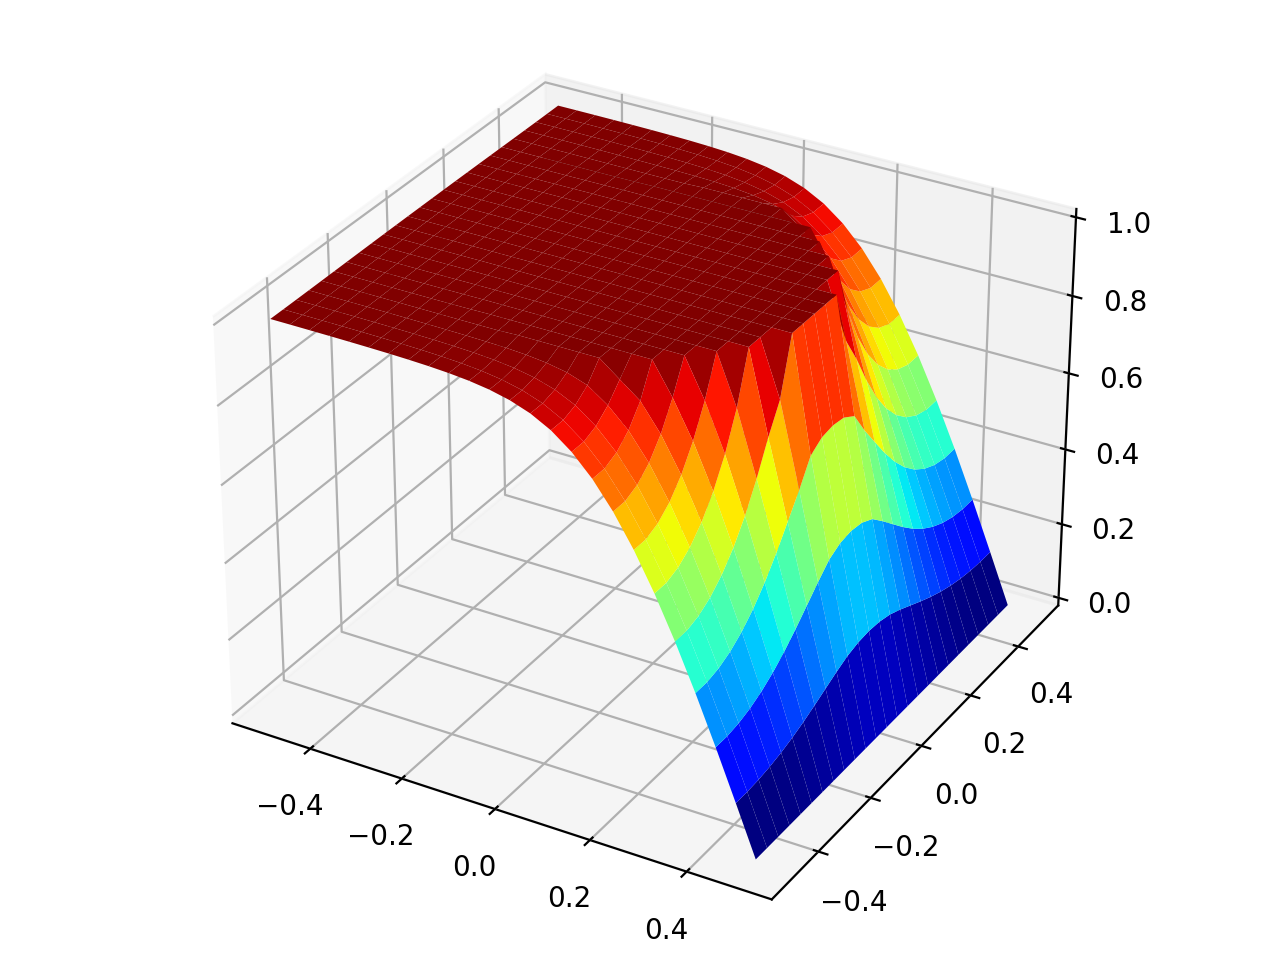
\includegraphics[scale=0.6]{Fig-6.png}
\caption{3d Plot of Potential}
\label{fig:2d Plot of Potential}
\end{figure}
\section{Calculating and Plotting current density}
The equations for current density in terms of potential is,
\begin{equation}
    J_x = -\partial\phi/\partial x
\end{equation}
\begin{equation}
    J_y = -\partial\phi/\partial y
\end{equation}
Here again we have to convert the differential equations to discrete domain. Thus,
\begin{equation}
    J_{x,ij} = 0.5*(\phi_{i,j-1} - \phi_{i,j+1})
\end{equation}
\begin{equation}
    J_{y,ij} = 0.5*(\phi_{i-1,j} - \phi_{i+1,j})
\end{equation}
\begin{lstlisting}
#finding and plotting current density
Jx,Jy = (1/2*(phi_matrix[1:-1,0:-2]-phi_matrix[1:-1,2:]), 1/2*(phi_matrix[:-2,1:-1]-phi_matrix[2:,1:-1]))
plt.title("Vector plot of current flow")
plt.quiver(Y[1:-1,1:-1],-X[1:-1,1:-1],-Jx[:,::-1],-Jy)
x_electrode,y_electrode=np.where(X**2+Y**2<(0.35)**2)   #Points with electode
plt.plot((x_electrode-Nx/2)/Nx,(y_electrode-Ny/2)/Ny,'ro')  #Mark those points as red
plt.show()
\end{lstlisting}
\begin{figure}[h!]
\centering
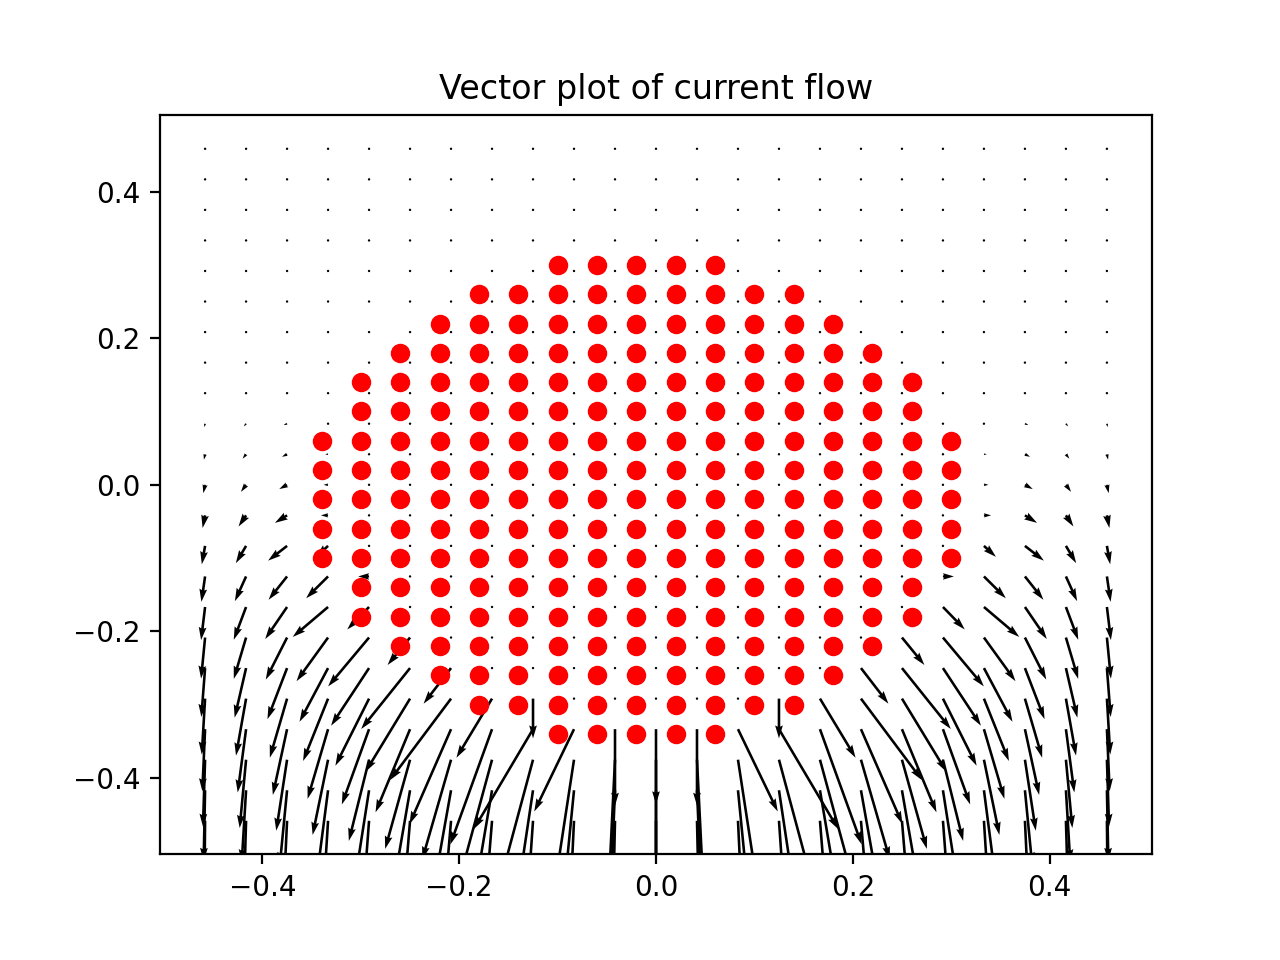
\includegraphics[scale=0.6]{Fig-7.png}
\caption{Vector plot of current flow}
\label{Vector plot of current flow}
\end{figure}
\section{Finding temperature at different regions on the plate}
Using the Laplace equation for heat flow,
\begin{equation}
    \nabla^2 T = -\frac{q}{\kappa} = -\frac{|J|^2}{\sigma \kappa}
\end{equation}
we find the temperature at various points on the plate.

This is very similar to the potential case, except for different initial values.
\begin{lstlisting}
#Function to update temperature matrix
def update_phi_temperature(temp,oldtemp,Jx,Jy):
    temp[1:-1,1:-1]=0.25*(tempold[1:-1,0:-2]+ tempold[1:-1,2:]+ tempold[0:-2,1:-1] + tempold[2:,1:-1]+(Jx)**2 +(Jy)**2)
    return temp


#Function to set boundary conditions for temperature matrix
def set_boundary_conditions_temperature(phi_matrix):
    phi_matrix[:,Nx-1]=phi_matrix[:,Nx-2] # Right Boundary
    phi_matrix[:,0]=phi_matrix[:,1] # Left Boundary
    phi_matrix[0,:]=phi_matrix[1,:] # Top Boundary
    phi_matrix[Ny-1,:]=300.0
    center = np.where(X**2+Y**2<(0.35)**2)
    phi_matrix[center]=300.0    #Make electode temperature as 300K
    return phi_matrix

#initialize temperature matrix
temp=300 * np.ones((Nx,Ny),dtype = float)

#Iterate and update the temperature matrix
for k in range(Niter):
    tempold = temp.copy()
    temp = update_phi_temperature(temp,tempold,Jx,Jy)   #Update step
    temp = set_boundary_conditions_temperature(temp)    #Set boundary condition after every iteration


#plotting 2d contour of final temp
plt.title("Contour plot of temperature")
plt.xlabel(r"X$\longrightarrow$")
plt.ylabel(r"Y$\longrightarrow$")
x_electrode,y_electrode=np.where(X**2+Y**2<(0.35)**2)   #Points with electode
plt.plot((x_electrode-Nx/2)/Nx,(y_electrode-Ny/2)/Ny,'ro')  #Mark those points as red
plt.contourf(Y,X[::-1],temp)
plt.colorbar()
plt.show()
\end{lstlisting}

\begin{figure}[h!]
\centering
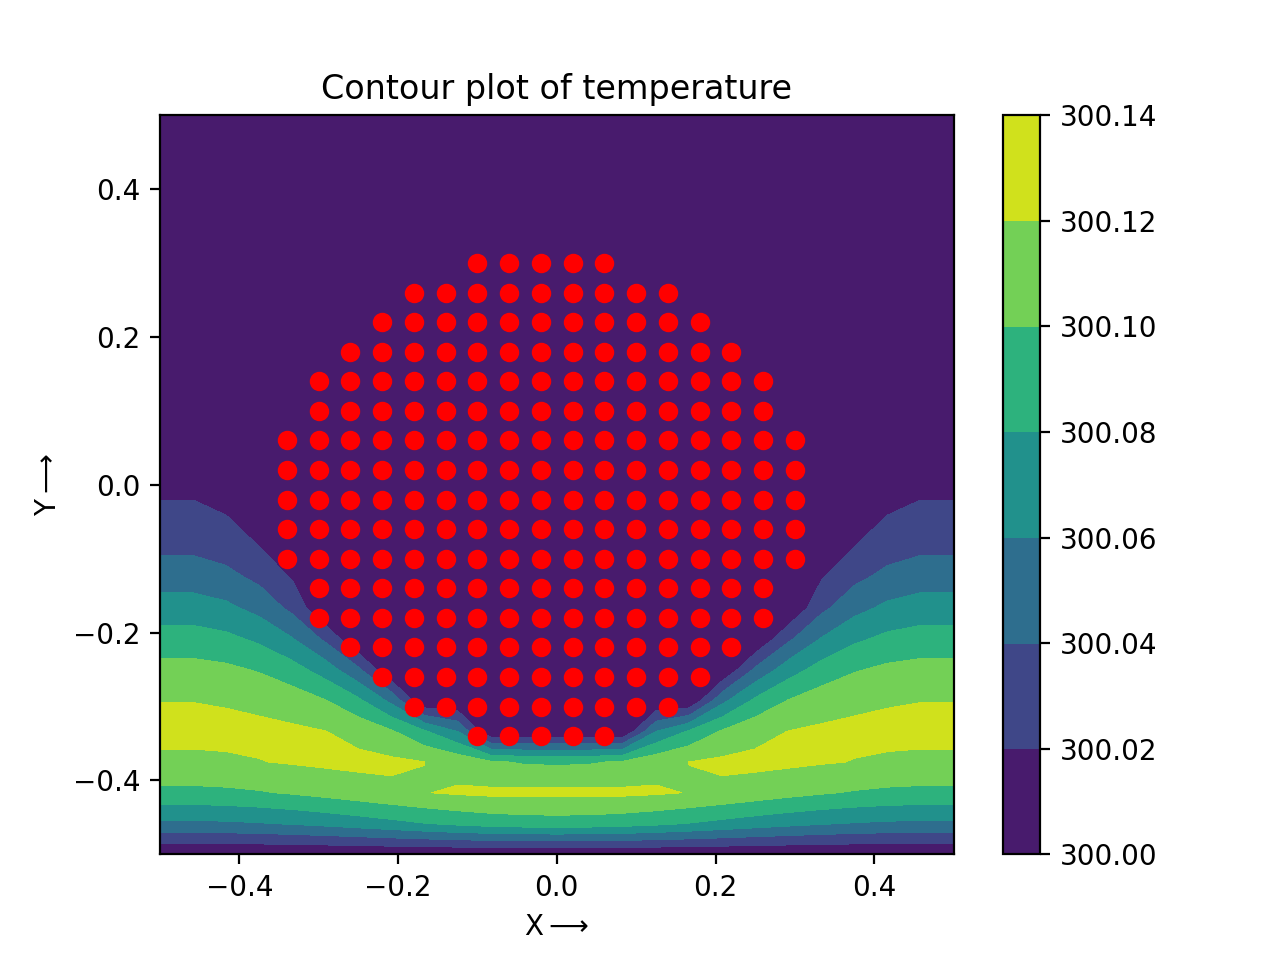
\includegraphics[scale=0.6]{Fig-8.png}
\caption{Cumulative error values on a log log scale}
\label{fig:3d Plot of Potential}
\end{figure}


\section{Conclusion}
We thus solved Laplace's equation using difference in discrete domain by iterating it over and over again. We also learnt to use vectorized code in python. Also this method is pretty poor in the sense that the error reduces pretty slowly with the iterations.

\end{document}
